\documentclass[12pt]{article}
\usepackage[paper=letterpaper,margin=2cm]{geometry}
\usepackage{amsmath,amssymb,amsfonts}
\usepackage{enumitem}
\usepackage{titling}
\usepackage{multirow}
\usepackage{xcolor}
\usepackage{float}
\usepackage{graphicx}
\usepackage{xcolor}
\definecolor{ISTBlue}{RGB}{0, 139, 255}
\usepackage[colorlinks=true, linkcolor=red]{hyperref}
\usepackage{subcaption} % For subfigures
\usepackage{adjustbox}  % For centering the bottom image


\setlength{\droptitle}{-6em}

\begin{document}

\begin{center}
Aprendizagem 2023\\
Homework I --- Group 003\\
(ist1107028, ist1107137)\vskip 1cm
\end{center}

\large{\textbf{Part I}: Pen and paper}\normalsize

\begin{enumerate}[leftmargin=\labelsep]
\item \textbf{Complete the given decision tree using Shannon entropy ($\log_2$) and considering that:
    (i) a minimum of 4 observations is required to split an internal node, and (ii) decisions by ascending alphabetic should be placed in case of ties.}

\vspace{1em}
The entropy of $y_\text{out}$ is given by:

\begin{equation*}
    \begin{split}
        H(y_{\text{out}}|y_1 >= 0.3) = - P(y_{\text{out}} = A|y_1 >= 0.3)\log_2(P(y_{\text{out}} = A|y_1 >= 0.3)) \\
        H(y_{\text{out}}|y_1 >= 0.3) = - P(y_{\text{out}} = B|y_1 >= 0.3)\log_2(P(y_{\text{out}} = B|y_1 >= 0.3)) \\
        H(y_{\text{out}}|y_1 >= 0.3) = - P(y_{\text{out}} = C|y_1 >= 0.3)\log_2(P(y_{\text{out}} = C|y_1 >= 0.3)) \\
    \end{split}
\end{equation*}

Replacing by the values is obtained:

\begin{equation*}
    H(y_{\text{out}}|y_1 >= 0.3) = - \left( \frac{3}{7} \log_2 \left( \frac{3}{7} \right) + \frac{2}{7} \log_2 \left( \frac{2}{7} \right) + \frac{2}{7} \log_2 \left( \frac{2}{7} \right) \right) \approx  1.5567
\end{equation*}

\vspace{0.5em}
We must now calculate $H(y_{\text{out}} | y_1 >= 0.3, y_x)$, in wich x will assume the values of 2, 3 and 4:

\begin{equation}
    \label{H-y_out}
    \begin{split}
    H(y_{\text{out}} | y_1 >= 0.3, y_x) = P(y_x = 0 | y_1 >= 0.3) H(y_{\text{out}} | y_1 >= 0.3, y_x = 0) \\
    + P(y_x = 1 | y_1 >= 0.3) H(y_{\text{out}} | y_1 >= 0.3, y_x = 1) \\
    + P(y_x = 2 | y_1 >= 0.3) H(y_{\text{out}} | y_1 >= 0.3, y_x = 2)
    \end{split}
\end{equation}

The information gain of $y_x$ is given by:

\begin{equation}\label{IG}
    IG(y_{\text{out}} | y_1 >= 0.3, y_x) = H(y_{\text{out}} | y_1 >= 0.3) - H(y_{\text{out}} | y_1 >= 0.3, y_x)
\end{equation}

\vspace{0.2cm}
\fbox{x=2:}

\begin{equation*}
    P(y_2 = 0 | y_1 >= 0.3) = \frac{4}{7} \quad
    P(y_2 = 1 | y_1 >= 0.3) = \frac{3}{7} \quad
    P(y_2 = 2 | y_1 >= 0.3) = \frac{0}{7} \quad
\end{equation*}

\begin{equation*}
    \begin{aligned}
        H(y_{\text{out}} | y_1 > 0.3, y_2 = 0) &= - \left( \frac{1}{4} \log_2 \left( \frac{1}{4} \right) + \frac{1}{4} \log_2 \left( \frac{1}{4} \right) + \frac{2}{4} \log_2 \left( \frac{2}{4} \right) \right) = 1.5
        \\
        H(y_{\text{out}} | y_1 > 0.3, y_2 = 1) &= - \left( \frac{2}{3} \log_2 \left( \frac{2}{3} \right) + \frac{1}{3} \log_2 \left( \frac{1}{3} \right) + \frac{0}{3} \log_2 \left( \frac{0}{3} \right) \right) \approx 0.9183
        \\
        %H(y_{\text{out}} | y_1 > 0.3, y_2 = 2) &= - \left( \frac{0}{0} \log_2 \left( \frac{0}{0} \right) + \frac{0}{0} \log_2 \left( \frac{0}{0} \right) + \frac{0}{0} \log_2 \left( \frac{0}{0} \right) \right) = 0
        %\\
    \end{aligned}
\end{equation*}

\newpage
On account of the fact that $P(y_2 = 2 | y_1 >= 0.3) = \frac{0}{7} = 0$, $H(y_{\text{out}} | y_1 > 0.3, y_2 = 2)$ will also be 0.\\

Thus, by inserting these values into equation \eqref{H-y_out}, we get:

\begin{equation*}
    H(y_{\text{out}} | y_1 >= 0.3, y_2) = \frac{4}{7} \times 1.5 + \frac{3}{7} \times 0.9183 + \frac{0}{7} \times 0 = 1.2507
    \\
\end{equation*}
\\
Lastly, we calculate the information gain as per \eqref{IG}:

\begin{equation*}
    IG(y_{\text{out}} | y_1 >= 0.3, y_2) = 1.5567 - 1.2507 = 0.306
\end{equation*}

\fbox{x=3:}
\begin{equation*}
    P(y_3 = 0|y_1 >= 0.3) = \frac{2}{7} \quad
    P(y_3 = 1|y_1 >= 0.3) = \frac{4}{7} \quad
    P(y_3 = 2|y_1 >= 0.3) = \frac{1}{7} \quad
\end{equation*}

\begin{equation*}
    \begin{aligned}
        H(y_{\text{out}}|y_1 >= 0.3, y_3 = 0) = - \left( \frac{2}{2} \log_2 \left( \frac{2}{2} \right) + \frac{0}{2} \log_2 \left( \frac{0}{2} \right) + \frac{0}{2} \log_2 \left( \frac{0}{2} \right) \right) &= 0 
        \\
        H(y_{\text{out}}|y_1 >= 0.3, y_3 = 1) = - \left( \frac{1}{4} \log_2 \left( \frac{1}{4} \right) + \frac{1}{4} \log_2 \left( \frac{1}{4} \right) + \frac{2}{4} \log_2 \left( \frac{2}{4} \right) \right) &= 1.5
        \\
        H(y_{\text{out}}|y_1 >= 0.3, y_3 = 2) = - \left( \frac{0}{1} \log_2 \left( \frac{0}{1} \right) + \frac{1}{1} \log_2 \left( \frac{1}{1} \right) + \frac{0}{1} \log_2 \left( \frac{0}{1} \right) \right) &= 0
    \end{aligned}
\end{equation*}

Thus, by inserting these values into equation \eqref{H-y_out}, we get:

\begin{equation*}
    H(y_{\text{out}}|y_1 >= 0.3, y_3) = \frac{2}{7} \times  0 + \frac{4}{7} \times 1.5 + \frac{1}{7} \times 0 \approx 0.8571 
\end{equation*}
\\
Lastly, we calculate the information gain as per \eqref{IG}:

\begin{equation*}
    IG(y_{\text{out}} | y_1 >= 0.3, y_3) = 1.5567 - 0.8571 = \textbf{0.6996}
\end{equation*}

\fbox{x=4:}
\begin{equation*}
    P(y_4 = 0|y_1 >= 0.3) = \frac{4}{7} \quad
    P(y_4 = 1|y_1 >= 0.3) = \frac{3}{7} \quad
    P(y_4 = 2|y_1 >= 0.3) = \frac{0}{7} \quad
\end{equation*}

\begin{equation*}
    \begin{aligned}
        H(y_{\text{out}}|y_1 >= 0.3, y_4 = 0) = - \left( \frac{2}{4} \log_2 \left( \frac{2}{4} \right) + \frac{2}{4} \log_2 \left( \frac{2}{4} \right) + \frac{0}{4} \log_2 \left( \frac{0}{4} \right) \right) &= 1 
        \\
        H(y_{\text{out}}|y_1 >= 0.3, y_4 = 1) = - \left( \frac{1}{3} \log_2 \left( \frac{1}{3} \right) + \frac{0}{3} \log_2 \left( \frac{0}{3} \right) + \frac{2}{3} \log_2 \left( \frac{2}{3} \right) \right) &\approx 0.9183
        \\
    \end{aligned}
\end{equation*}

\newpage

Once again,  $P(y_4 = 2 | y_1 >= 0.3) = \frac{0}{7} = 0$. Therefore $H(y_{\text{out}} | y_1 > 0.3, y_4 = 2)$ will also equal 0.\\

Thus, by inserting these values into equation \eqref{H-y_out}, we get:

\begin{equation*}
    H(y_{\text{out}}|y_1 >= 0.3, y_4) = \frac{4}{7} \times 1 + \frac{3}{7} \times 0.9183 + \frac{0}{7} \times 0 \approx 0.9650
\end{equation*}
\\
Lastly, we calculate the information gain as per \eqref{IG}:

\begin{equation*}
    IG(y_{\text{out}} | y_1 >= 0.3, y_4) = 1.5567 - 0.9650 = 0.5917
\end{equation*}

\vspace{0.5cm}

\hspace*{2em}After calculating the information gains for each attribute, we can observe that the attribute $y_3$ has the highest value of 0.6996. 
Accordingly, we chose it as the next node. Since there are at least four observations with $y_1 >= 0.3$, we split the new node. 

\hspace*{2em}If we fix $y_1 >= 0.3$ with $y_3 = 0$, $y_3 = 1$ and $y_3 = 2$, we will obtain 2, 4 and 1 observations, respectively. This gives us three new leaves for the branch in question. The node corresponding to $y_3 = 0$ will be class A, and the one corresponding to $y_3 = 2$ will be from class B, since these classes are the ones that appear most frequently for the respective conditions in the data set.
For the $y_3 = 2$ branch with the $y_1 >= 0.3$  condition we get exactly four observations, as we said previously. That being the case, we must split the next node with the higher information gain. 

\[
    \begin{aligned}
    H(y_{\text{out}} | y_1 >= 0.3 , y_3 = 1, y_2 = 0) & = - \left(\frac{1}{4} \log_2\left(\frac{1}{4}\right) + \frac{1}{4} \log_2\left(\frac{1}{4}\right)
    + \frac{2}{4} \log_2\left(\frac{2}{4}\right)\right) = 1.5                                                                       \\
    H(y_{\text{out}} | y_1 >= 0.3 , y_3 = 1, y_2 = 1) & = - \left(\frac{0}{0} \log_2\left(\frac{0}{0}\right) + \frac{0}{0} \log_2\left(\frac{0}{0}\right)
    + \frac{0}{0} \log_2\left(\frac{0}{0}\right)\right) = 0                                                                     \\
    H(y_{\text{out}} | y_1 >= 0.3 , y_3 = 1, y_2 = 2) & = - \left(\frac{0}{0} \log_2\left(\frac{0}{0}\right) + \frac{0}{0} \log_2\left(\frac{0}{0}\right)
    + \frac{0}{0} \log_2\left(\frac{0}{0}\right)\right) = 0                                                                       \\
    H(y_{\text{out}} | y_1 >= 0.3 , y_3 = 1, y_4 = 0) & = - \left(\frac{0}{1} \log_2\left(\frac{0}{1}\right) + \frac{1}{1} \log_2\left(\frac{1}{1}\right)
    + \frac{0}{1} \log_2\left(\frac{0}{1}\right)\right) = 0                                                                       \\
    H(y_{\text{out}} | y_1 >= 0.3 , y_3 = 1, y_4 = 1) & = - \left(\frac{1}{3} \log_2\left(\frac{1}{3}\right) + \frac{0}{3} \log_2\left(\frac{0}{3}\right)
    + \frac{2}{3} \log_2\left(\frac{2}{3}\right)\right) = 0.9183                                                                      \\
    H(y_{\text{out}} | y_1 >= 0.3 , y_3 = 1, y_4 = 2) & = - \left(\frac{0}{0} \log_2\left(\frac{0}{0}\right) + \frac{0}{0} \log_2\left(\frac{0}{0}\right)
    + \frac{0}{0} \log_2\left(\frac{0}{0}\right)\right) = 0 
    \end{aligned}
    \]

    From other calculations above, we know that:

    \[
        H(y_{\text{out}} | y_1 >= 0.3 , y_3 = 1) = 1.5
    \]

    Therefore, replacing the above values on equation \eqref{H-y_out}, gives us:

    \[
        \begin{aligned}
        E(y_{\text{out}} | y_1 >= 0.3, y_3 = 1, y_2) & = \frac{4}{4} \times 1.5 + \frac{0}{4} \times 0 + \frac{0}{4} \times 0 = 1.5  \\
        E(y_{\text{out}} | y_1 >= 0.3, y_3 = 1, y_4) & = \frac{1}{4} \times 0 + \frac{3}{4} \times 0.9183 + \frac{0}{4} \times 0 = 0.6887
        \end{aligned}
    \]

    Finally, we can calculate the information gain, as per \eqref{IG}:

    \[
        \begin{aligned}
        IG(y_{\text{out}} |y_1 >= 0.3, y_3 = 1, y_2) & = 1.5 - 1.5 = 0 \\
        IG(y_{\text{out}} |y_1 >= 0.3, y_3 = 1, y_4) & = 1.5 - 0.6887 = \textbf{0.8113}
        \end{aligned}
    \]
\\

Since $y_4$ is the node with the highest information gain of 0.8113, it is the node we chose to split. With the conditions of $y_1 >= 0.3$ and $y_3 = 1$, we can check that the conditions $y_4 = 0$, $y_4 = 1$ and $y_4 = 2$ all have less than 4 observations each. Therefore, we take the class with the highest frequency
for each respective conditions on the dataset.
Finally, we can construct the following decision tree:

\begin{figure}[H]
          \centering
          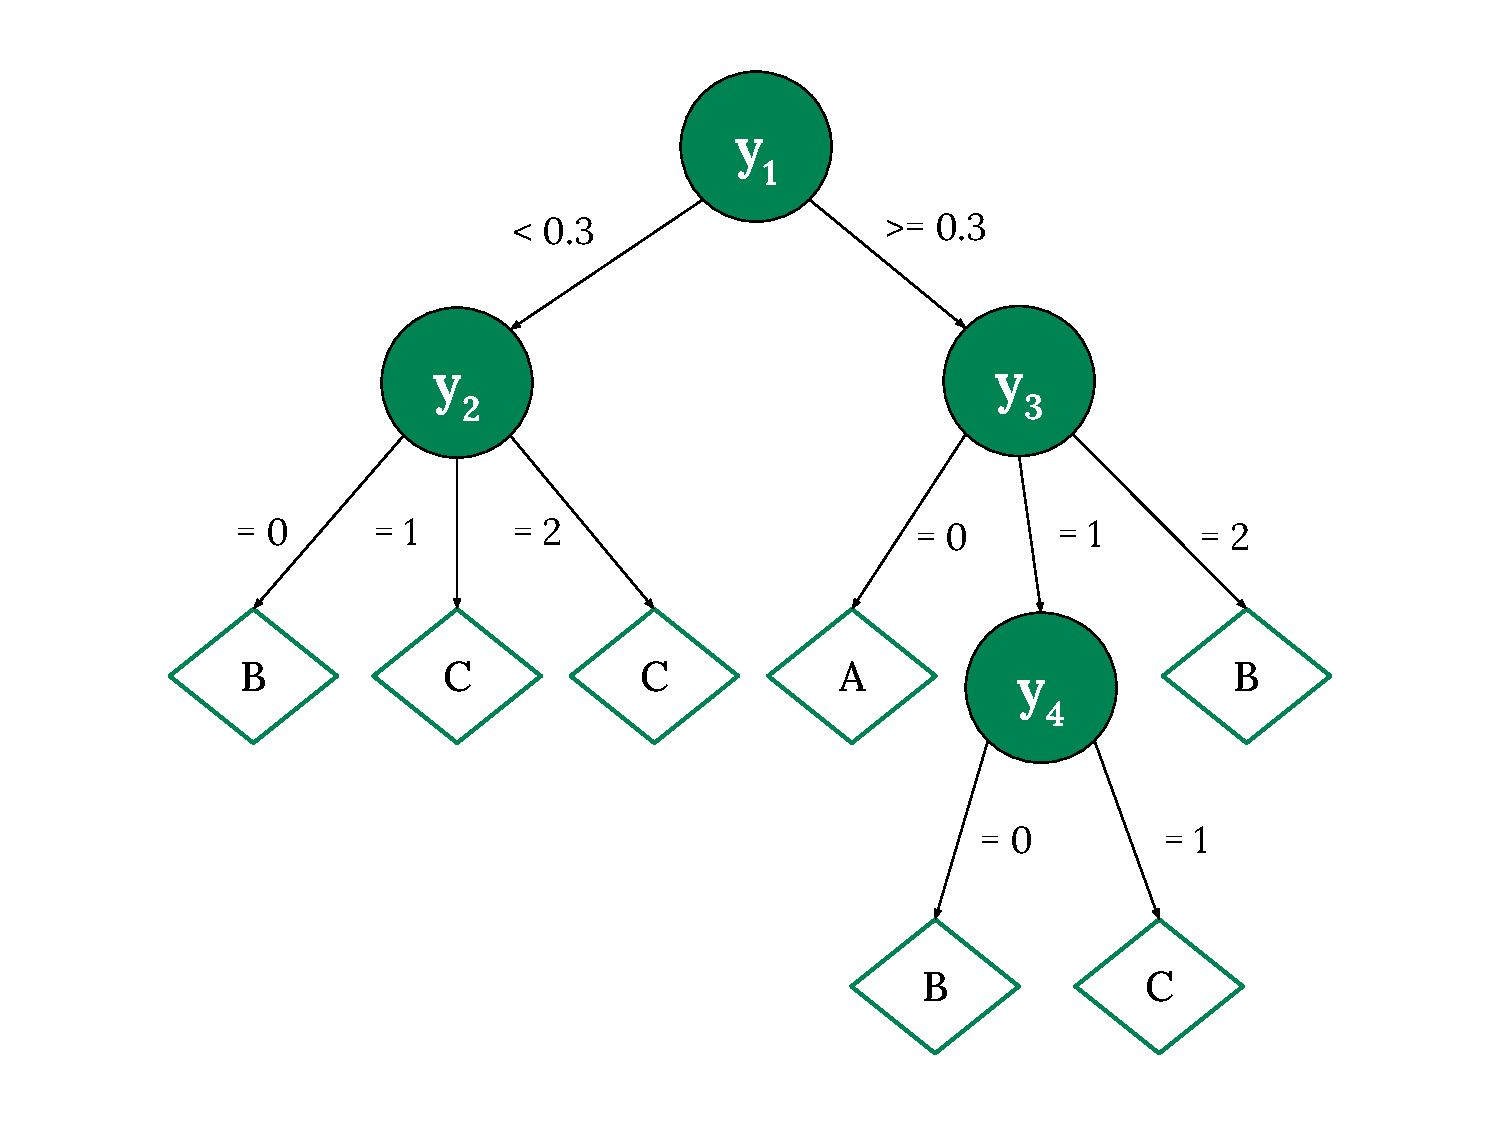
\includegraphics[width=15cm]{Decision Tree.pdf}
          \caption{Decision Tree for exercise 1}
          \label{fig:decision_tree}
        \end{figure}

\newpage

\item \textbf{Draw the training confusion matrix for the learnt decision tree.}

\vspace{1em}
We can then predict the values for each observation through the decision tree drawn in the previous point.\\

To do this, we start at the initial node of the tree and follow its branches. When we reach the next node, the process is repeated for the succeeding variable and the following ones until a leaf is reached.
The class present in this leaf will correspond to the predicted value for the respective D. The real value will be the one in the $y_out$ column corresponding to that same D.\\

This results in the following values:

\begin{center}
    \begin{tabular}{cccccccccccccc}
        \multicolumn{2}{c}{}  $x_1$ & $x_2$ & $x_3$ & $x_4$ & $x_5$ & $x_6$ & $x_7$ & $x_8$ & $x_9$ & $x_{10}$ & $x_{11}$ & $x_{12}$ \\
        \multirow{1}{*}{real}      & =    [ C & B & C & B & C & B & A & A & C & C & A & B  ] \\
        \multirow{1}{*}{predicted} & =   [ C & B & C & B & C & B & \textcolor{red}{C} & A & C & C & A & B  ]
  \end{tabular}
\end{center}

\vspace{0.2cm}
Finally, we set up the confusion matrix by counting the pairs of observations previously mentioned.

\vspace{0.2cm}

\begin{figure}[H]
          \centering
          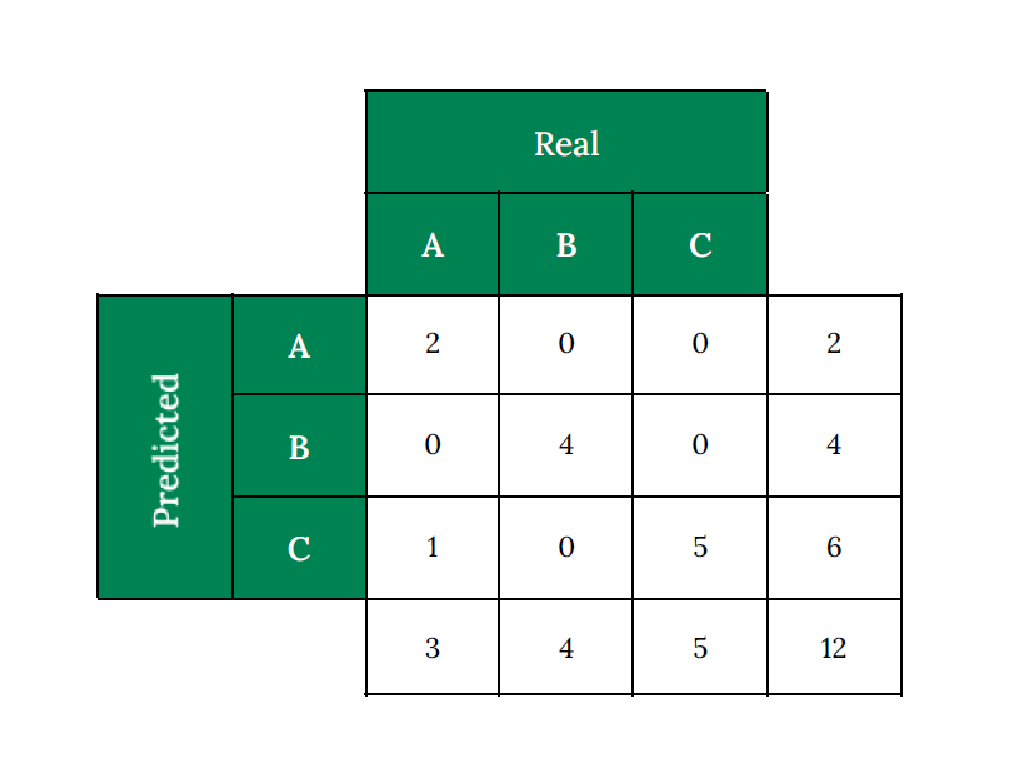
\includegraphics[width=9.5cm]{Confusion Matrix.pdf}
          \caption{Confusion matrix for exercise 2}
          \label{fig:Confusion matrix}
        \end{figure}

\vspace{0.5cm}

\item \textbf{Identify which class has the lowest training F1 score.} 

\vspace{1em}

\(\text{F1}_{\text{score}}\) is given by the following equation:

    \begin{equation}\label{ex3-f1}
        \text{F1}_{\text{score}} = 2 \times \frac{{\text{Precision} \times \text{Recall}}}{{\text{Precision} + \text{Recall}}}
    \end{equation}

\newpage

And precision and recall are given by:

    \begin{equation}\label{e3-p}
        \text{Precision} = \frac{\text{True Positives}}{{\text{True Positives}
        \text{False Positives}}}
    \end{equation}

    \begin{equation}\label{e3-r}
        \text{Recall} = \frac{\text{True Positives}}{{\text{True Positives} + \text{False Negatives}}}
    \end{equation}
\\

We can calculate the precision by replacing the according values for each class in equation \eqref{e3-p}:

    \begin{equation*}
        \text{Precision}_A = \frac{2}{2+0} = 1 \qquad
        \text{Precision}_B = \frac{4}{4+0} = 1 \qquad
        \text{Precision}_C = \frac{5}{5+1} = \frac{5}{6}
    \end{equation*}
\\

Same goes for recall, using equation \eqref{e3-r}:

    \begin{equation*}
        \text{Recall}_A = \frac{2}{2+1} =  \frac{2}{3}\qquad
        \text{Recall}_B = \frac{4}{4+0} = 1\qquad
        \text{Recall}_C = \frac{5}{5+0} = 1
    \end{equation*}
\\

At Last, we determine each \(\text{F1}_{\text{score}}\) with \eqref{ex3-f1}:

    \begin{equation*}
        \displaystyle
        {\text{F1}_{\text{score}}}_A = 2 \times \frac{{ 1 \times \frac{2}{3} }}{{  1 + \frac{2}{3} }} = 0.8000 \qquad
        {\text{F1}_{\text{score}}}_B = 2 \times \frac{{ 1 \times 1 }}{{ 1 + 1 }} = 1  \qquad
        {\text{F1}_{\text{score}}}_C = 2 \times \frac{{ \frac{5}{6} \times 1 }}{{ \frac{5}{6} + 1 }} \approx 0.9091 
    \end{equation*}
\\

The \textbf{class with the lowest training F1 score is A}, with a score of 0.8000.

% Até este ponto já está tudo ok, mas é melhor rever

\vspace{1cm}

\item  \textbf{Draw the class-conditional relative histograms of y1 using 5 equally spaced bins in
[0,1]. Find the n-ary root split using the discriminant rules from these empirical
distributions.}

\end{enumerate}
\begin{enumerate}
    \item First step for this problem was creating a histogram for every class present, which are A, B and C. For each, when a value of $y_1$ falls into a bin, we add one to the value of that bin. Each bin has a size of 0.2, since we are using 5 equal spaced bins in the interval [0,1].

        \begin{figure}[ht]
    \centering
    % Top row: two images side by side
    \begin{minipage}[t]{0.48\linewidth}
        \centering
        \fbox{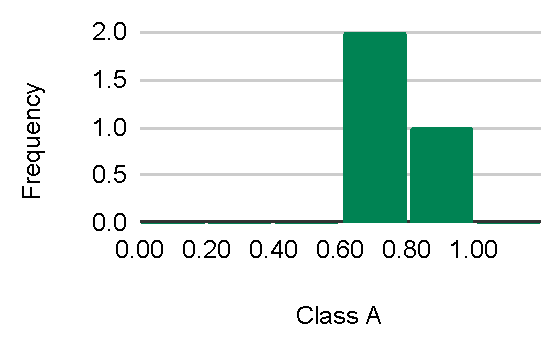
\includegraphics[width=\linewidth]{ClassA.pdf}}
        \subcaption{Histogram for Class A}
    \end{minipage}
    \hfill
    \begin{minipage}[t]{0.48\linewidth}
        \centering
        \fbox{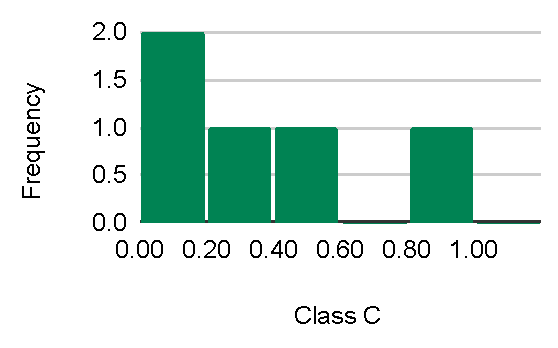
\includegraphics[width=\linewidth]{ClassB.pdf}}
        \subcaption{Histogram for Class B}
    \end{minipage}
    
    % Spacer between top and bottom row
    \vspace{0.5cm} % Adjust this value as needed

    % Bottom image centered
    \begin{minipage}[t]{0.48\linewidth}
        \centering
        \fbox{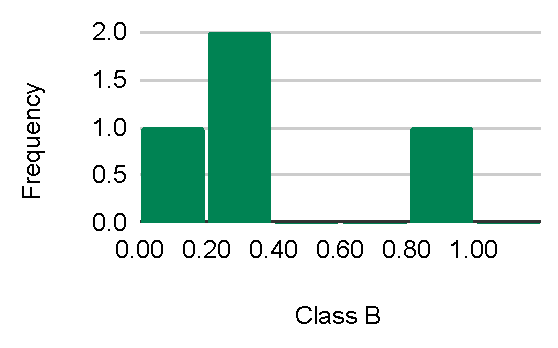
\includegraphics[width=\linewidth]{ClassC.pdf}}
        \subcaption{Histogram for Class C}
    \end{minipage}
    
    \caption{Class-conditional relative histograms of $y_1$ using 5 equal spaced bins in [0,1]}
\end{figure}

\vspace{10cm}

\item For a quick and broad overview of how to create documents in {\LaTeX} see 
\end{enumerate}

\newpage

\large{\textbf{Part II}: Programming}\normalsize

\begin{enumerate}[leftmargin=\labelsep,resume]
\item Solution to the programming questions here.
\end{enumerate}     
\vskip 1cm
\textbf{End note}: do not forget to also submit your Jupyter notebook

\end{document}
